\subsection{Model Evaluation,Validation and Justification}
%The final model’s qualities — such as parameters — are evaluated in detail. Some type of analysis is used to validate the robustness of the model’s solution.

By utilizing the bayesian optimization, I optimized the number of dimensions of first layer of fully connected layer and learning rate. I got the optimal number of first layer of fully connected layer and the learning rate of the optimizer.Those numbers are 204 and 0.000597,respectively. By using those numbers, I got the test accuracy which is 72.1\%


From the result of Bayesian Optimization, I chose 204 of first fully connected layer and 0.000597 of learning rate as the final model parameters.


The training and test accuracy in this model is as follows(Fig.13).


\begin{figure}[H]

	\begin{center}
	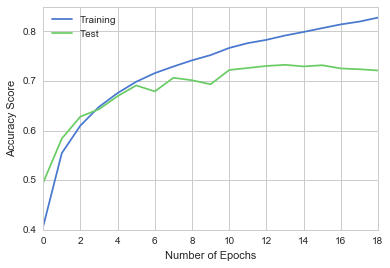
\includegraphics[width=5cm]{picture/final_model_accuracy.png}
	\caption{Accuracy rate of training and validation data}
	\end{center}
	\label{fig:13}

\end{figure}


The loss of the model is shown in Fig.14

 \begin{figure}[H]

	\begin{center}
	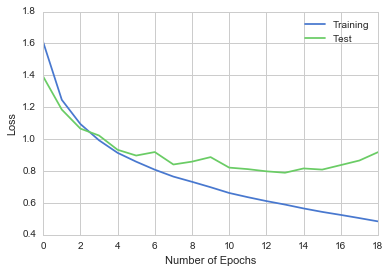
\includegraphics[width=5cm]{picture/final_loss.png}
	\caption{Loss of training and validation data}
	\end{center}
	\label{fig:14}

\end{figure}



%The final results are compared to the benchmark result or threshold with some type of statistical analysis. Justification is made as to whether the final model and solution is significant enough to have adequately solved the problem.

The model improves the accuracy rate by 2.0\%. The final model doesn't seem to fall into the overfitting according to the Fig.13 and when compared to the Fig.11 which is the benchmark result, the difference between the training and test accuracy rate is much smaller. That means the final model is more robust than the benchmark model. Therefore, the model improved compared to the benchmark result.


%The training and validation loss in the benchmark is Fig---. The counterpart in final result is Fig.---


%The number of miss-classified data in benchmark is ----. On the other hand, the number in the final result is ----.The distribution difference in miss-classified data between the benchmark and the final result is following.
